\chapter{Métodos Supervisados}
\pagenumbering{arabic}
%Supongamos que tenemos un conjunto de variables, $\textbf{X}$ que influyen sobre una o más variables conocidas $\textbf{Y}$. A partir de ahora, las llamaremos variables de entrada y variables objetivo respectivamente. El principal propósito de los métodos supervisados, es dado una muestra de individuos con observaciones de ambos tipos de variables predecir la variable objetivo para nuevos individuos de los que solo conozcamos las variables de entrada  
%
%Para empezar tenemos que fundamentar de manera teórica como calcular esa función para predecir. 

%\section{Teoría de decisión estadística}
Sea $X\in \mathbb{R}^p$ un vector aleatorio real e $Y \in \mathbb{R}$ una variable aleatoria real. En este contexto, $X$ e $Y$ serán las variables de entrada y la variable de salida respectivamente. Asimismo, sea $\mathbb{P}(X,Y)$ la distribución de probabilidad conjunta.   

Se busca una función $f(X)$ para predecir $Y$. Dicho predictor tiene asociada una pérdida, es decir, una forma de penalizar el error de predicción. En esta memoria, a no ser que se explicite utilizaremos el error cuadrático para las regresiones, $L(Y,f(X))=(Y-f(X))^2$ . 

\begin{defi}
Llamaremos error de predicción esperado de $f$ o $EPE(f)$ a la siguiente expresión:
\begin{equation}
EPE(f)=E(Y-f(X)^2)=\int (y-f(x))^2 \mathbb{P}(dx,dy)
\end{equation}

\noindent A priori se conocen los valores de $X$, entonces si condicionamos a dichos valores, obtenemos que $\mathbb{P}(Y,X)=\mathbb{P}(Y|X)\cdot\mathbb{P}(X)$ aplicándolo en la expresión anterior resulta que 
\begin{equation}
\begin{split}
EPE(f)&=\int (y-f(x))^2 \mathbb{P}(dx,dy)=\int\int (y-f(x))^2 \mathbb{P}(dy|dx)\mathbb{P}(dx)\\
&= \mathbb{E}_X(\mathbb{E}_{Y|X}((Y-f(X))^2|X))
\end{split}
\end{equation}

\end{defi}

\noindent Este parámetro nos ofrece un criterio para encontrar $f$, es decir, $f$ será la que minimice el $EPE(f)$ , en concreto, $f(x)=\mathbb{E}(Y|X=x)$. Añadir que este sería el caso de la regresión. 

\noindent No obstante, para los casos de \textbf{clasificación} cambia el hecho de que la función cuadrática de pérdida no es adecuada. Sea $G$ una variable categórica con $K$ distintos valores posibles, entonces su función de pérdida se puede expresar como una matriz \textbf{L}. Podemos definir el termino $l_{i,j}=$``Pérdida de clasificar como $G_i$ lo que en realidad es  $G_j$". Lo más frecuente es tomar la pérdida $0-1$, esta asigna 0 a las muestras correctamente clasificadas y 1 a las no categorizadas de manera satisfactoria. 

\noindent Con esta función de pérdida el error de predicción esperado pasa a ser: 


%\input{Documentos Extra/Regresion Lineal Multiple.tex}

%\input{Documentos Extra/Clasificacion Lineal Multiple.tex}

\newpage
\section{Redes Neuronales}

\noindent Las redes neuronales artificiales, son modelos predictivos basados en el funcionamiento de las propias neuronas del cerebro que reciben señales de entradas de las neuronas con las cuales están conectadas, las procesan y envían el resultado a las neuronas con las que estén conectadas. 

\noindent La ventaja de este tipo de algoritmos es que en esencia, son un conjunto de parámetros y funciones de activación que pueden ser ajustados para cualquier tarea y cualquier tipo de función a aproximar solo hace falta la complejidad del modelo adecuada según \emph{Hornik, K., Stinchcombe, M., y  White, H.} \cite{Hornik 1989}.  

\noindent Una neurona artificial es mucho más simple que una neurona, \emph{López R., E. Balsa-Canto y E. Oñate} \cite{Roberto 2008} definen una neurona en términos matemáticos, pero antes hay que definir los siguientes conceptos, para los cuales se han utilizado como base \cite{Grossi 2007, Neural Designer}

\noindent Sea un vector aleatorio $\mathbf{x}$ de longitud $p$, llamamos datos de entrada a los números que se introducen en la neurona que pueden ser los propios valores observados de las 
\begin{defi}
Llamaremos \emph{pesos sinápticos} $\omega$ de una neurona, al vector de $p$ constantes que regulan la importancia de cada entrada en la neurona.  A este vector de pesos sinápticos se le puede añadir un término independiente que únicamente se sumará, se le llama \emph{sesgo} y se denota como $b$.
\end{defi}

\begin{defi}
Se llama \emph{función de activación}, $f$ de una neurona artificial a la función que transforma la suma ponderada de las entradas para obtener la salida. 

\noindent Las funciones de activación más habituales son; la función \emph{identidad} \emph{(En este caso, es como si se hiciera una simple suma ponderada de los datos de entrada)}, la función \emph{sigmoide}, la \emph{tangente hiperbólica} o la función \emph{lineal regularizada} para casos de regresión, es decir, en casos en los que la variable respuesta sea continua. En caso contrario, se pueden utilizar la \emph{función softmax} o la \emph{función de regresión logística} para casos discretos, ya que devuelven valores en el intervalo $[0,1]$ y se puede asociar con la probabilidad de pertenecer a una clase u otra. 
\end{defi}
\begin{defi}
Una \emph{neurona artificial} procesa una entrada $\textbf{x}$ de acuerdo con unos \emph{pesos sinápticos} $(b,\omega)$ que luego es transformada por una función de activación $f(\mathbf{x})$.

\noindent Una  vez definidos los elementos que forman una neurona artificial estos se utilizan de manera que se utiliza la función:
\begin{equation}
\begin{split}
g:\mathbb{R}^p &\longrightarrow \mathbb{R}\\
g(\textbf{x})&\longrightarrow g(\textbf{x};b,\omega)
\end{split}
\end{equation}
\begin{equation}
g(\textbf{x})=f\left(b+\sum_{i=1}^p \omega_i x_i\right)
\end{equation}
El siguiente diagrama proporciona una forma sencilla de entender el funcionamiento de dicho modelo, incluyendo la analogía de las neuronas biológicas. 
\end{defi}
\begin{center}
%%Hay que pedirle a Carlos que lo edite por que yo la verdad que no se 
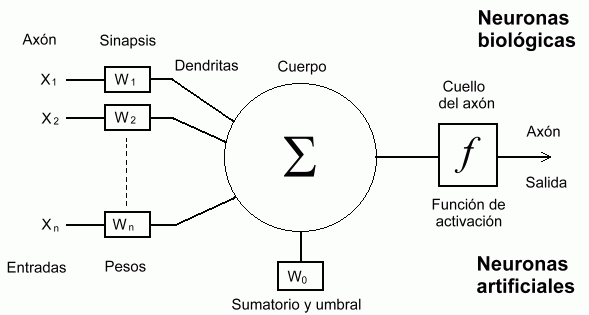
\includegraphics[scale=0.6]{Documentos Extra/Imagenes/neurona.png}
\end{center}

\noindent La principal ventaja de estos métodos es que las neuronas se pueden conectar entre ellas, es decir, estas se pueden organizar de manera que los datos de salida de un conjunto de neuronas sirvan como entrada del siguiente.
\begin{defi}
Se llama \emph{capa de neuronas} al conjunto de neuronas artificiales que tienen el mismo conjunto de datos de entrada y cuyos datos de salida para la siguiente.
\end{defi}
\noindent Se pueden establecer varios tipos de capas de neuronas \cite{Neural Designer}:
\begin{defi}
Se llama \emph{capa de entrada} a la primera capa de neuronas que recibe los valores de las observaciones y las estandariza (\emph{Se debe entrenar al modelo para ello}). Se establece una 
\end{defi}

\begin{defi}
Se llama \emph{capa oculta} a cada una de las capas intermedias que se utilizan en las redes neuronales. 
\end{defi}

\begin{defi}
Se llama \emph{capa de salida} a la última capa que tiene tantas neuronas como variables respuesta y sus datos de salida son las predicciones de 
\end{defi}

\noindent Para el proceso de ajuste se utiliza de manera habitual el método del gradiente con un conjunto de datos con $N$ observaciones. En el capitulo  11 \emph{Hastie et.al. }\cite{Hastie 2001} se detallan en profundidad el ajuste mediante el método del gradiente. De esta manera, se tiene un proceso que se llama \emph{back-propagation}. 

\noindent La siguiente imagen es una representación de una red neuornal como un grafo, en el que cada nodo es una neurona, en particular, los nodos azules son neuronas comunes, formando 5 capas ocultas, mientras que las amarillas son capas de escalado, y las rojas de salida. 

\begin{figure}[h]
\centering
%%Hay que pedirle a Carlos que lo edite por que yo la verdad que no se 
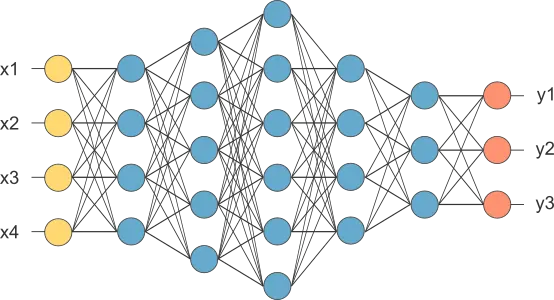
\includegraphics[scale=0.35]{Documentos Extra/Imagenes/red-neuronal-grande.png}
\caption{Imagen extraída directamente de www.neuraldesigner.com}
\end{figure}

\noindent Si se quisiera expresar el modelo como una única expresión, la expresión que se obtiene al hacer crecer un poco la red neuronal es bastante compleja de interpretar, por ejemplo en el caso anterior se tiene más de 100 parámetros y no es una red demasiado compleja, por tanto, la interpretación del modelo es compleja. Es por ello, que las redes neuronales se utilizan únicamente para fines predictivos \cite{Hastie 2001, James 2013}. 

\noindent Las principales ventajas de las redes neuronales es que pueden ajustarse a cualquier estructura sin conocerla a priori. Por otro lado, debido a la gran cantidad de parámetros a ajustar pueden provocar \emph{sobre-ajuste} pero para ello se pueden utilizar técnicas de validación cruzada \emph{(Capítulo 5 de \cite{James 2013} o el capítulo 7 de \cite{Hastie 2001})}

\noindent En esta memoria se han detallado los tipos más básicos de neuronas hay tareas específicas que este tipo de neuronas no pueden afrontar, por ejemplo, en el caso de datos que proceden de series temporales en las que estados previos influyen en los estados futuros como puede ser predicciones meteorológicas, bursátiles etc... se han desarrollado un tipo más complejo de neuronas llamadas LSTM \emph{(Long-Short Term Memory)} de las que se puede ver su desarrollo y definición además de las propiedades que poseen en \cite{Hochreiter 1997}. \emph{(Para una descripción más esquemática véase \cite{Neural Designer})}

